% Why We Backtest -- intuition for the Backtesting lecture.
% Figures and every number quoted here come from backtesting_intuition_figures.py
\documentclass[aspectratio=169,10pt]{beamer}
\usetheme{default}
\usecolortheme{default}

\usepackage{graphicx}
\usepackage{adjustbox}
\usepackage{amsmath}
\usepackage{amssymb}
\usepackage{booktabs}
\usepackage{appendixnumberbeamer}  % Exclude appendix from slide count

\setbeamertemplate{navigation symbols}{}
\setbeamertemplate{items}[circle]

% Footline: Author, Event (Year) on left; page/total on right
\setbeamertemplate{footline}{
  \hbox{%
    \begin{beamercolorbox}[wd=.5\paperwidth,ht=2.5ex,dp=1ex,left]{author in head/foot}%
      \hspace*{2ex}\insertshortauthor, \insertshortinstitute\ (\insertdate)
    \end{beamercolorbox}%
    \begin{beamercolorbox}[wd=.5\paperwidth,ht=2.5ex,dp=1ex,right]{date in head/foot}%
      \insertframenumber/\inserttotalframenumber\hspace*{2ex}
    \end{beamercolorbox}%
  }
}

% Highlight boxes
\setbeamercolor{box1}{bg=red!12,fg=black}

\title{Why We Backtest}
\subtitle{What a sample can tell you, and what it cannot}
\author[A. Moreira]{Alan Moreira}
\institute[Data-Driven Investing]{NYU Stern --- Data-Driven Investing}
\date{Fall 2026}

\begin{document}

%------------------------------------------------------------------ 1
\begin{frame}
\titlepage
\end{frame}

%------------------------------------------------------------------ 2
\begin{frame}[label=experiment]{An experiment}
Take 49 industry portfolios. Every December:
\vskip 12pt
\begin{enumerate}
\item Regress each industry on the market, using the last three years of daily returns
\[ r_t = \alpha + \beta\, r_{m,t} + \varepsilon_t \]
\item Buy the fifth with the highest $\alpha$, short the fifth with the lowest
\vskip 8pt
\item Hold for the next year
\end{enumerate}
\vskip 12pt
\textcolor{red}{Would that work?}
\hfill \hyperlink{appendix_a1}{\beamerbutton{Details}}
\end{frame}

%------------------------------------------------------------------ 3
\begin{frame}{Promised 26\%, delivered 2\%}
\begin{center}
\adjustbox{max width=0.80\textwidth, max height=0.40\textheight}{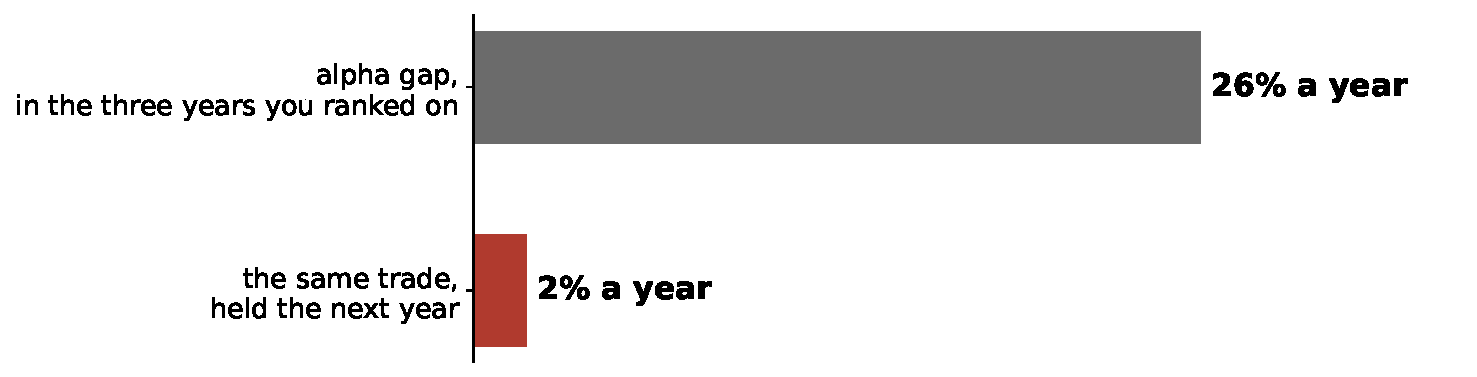
\includegraphics{figures/promised_vs_delivered.pdf}}
\end{center}
\vskip 1pt
\begin{itemize}
\item More than nine-tenths of the alpha you ranked on never showed up
\vskip 4pt
\item And 2\% a year is not distinguishable from zero: $t = 1.3$ over 97 years
\vskip 4pt
\item The trade is hedged: appraisal ratio $=$ average return $/$ volatility $= 1.9\% \,/\, 14.3\% = \textcolor{red}{0.13}$
\vskip 4pt
\item The same number from the $t$ and the sample size alone: $t \,/ \sqrt{T} = 1.3 \,/ \sqrt{97} = \textcolor{red}{0.13}$
\end{itemize}
\end{frame}

%------------------------------------------------------------------ 4
\begin{frame}{The other coefficient behaves}
\begin{center}
\adjustbox{max width=\textwidth, max height=0.70\textheight}{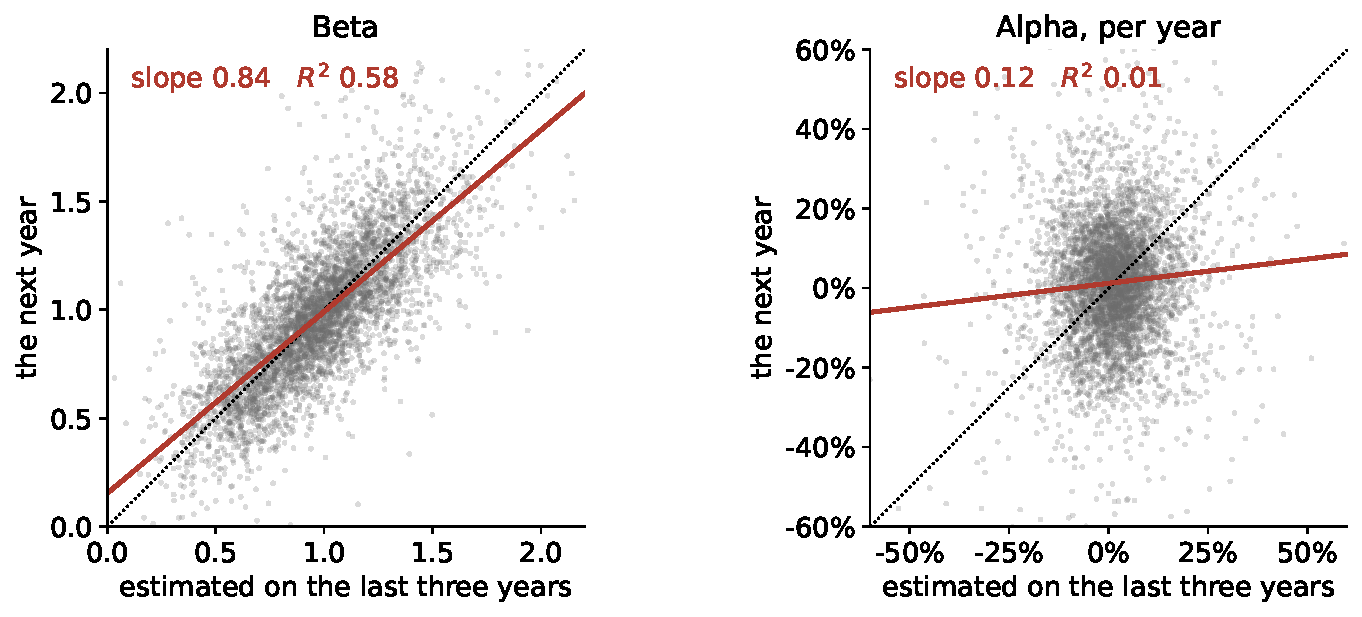
\includegraphics{figures/beta_alpha_persistence.pdf}}
\end{center}
\vskip 2pt
\begin{itemize}
\item Same regression, same three years. \textcolor{red}{Beta carries over; alpha does not.}
\end{itemize}
\end{frame}

%------------------------------------------------------------------ 5
\begin{frame}{So a hedge built in advance works}
\begin{center}
\adjustbox{max width=\textwidth, max height=0.68\textheight}{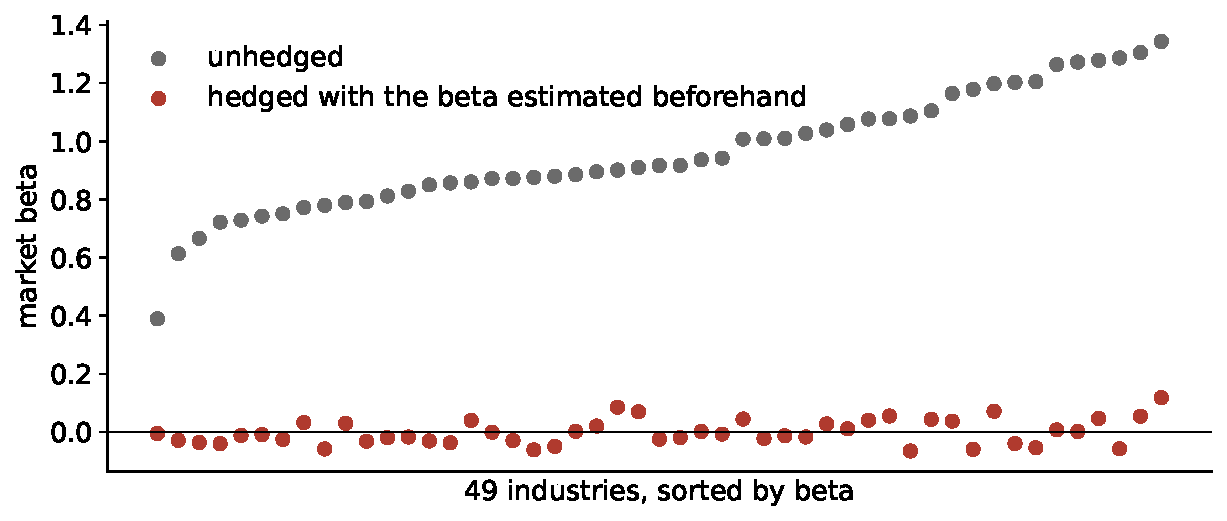
\includegraphics{figures/hedge_works.pdf}}
\end{center}
\vskip 2pt
\begin{itemize}
\item Hedge set before the year starts: betas of 0.39 to 1.34 fall to \textcolor{red}{0.03} on average
\end{itemize}
\end{frame}

%------------------------------------------------------------------ 6
\begin{frame}{Three years measure beta, not alpha}
49 industries, three years of daily data each, 1927--2025:
\vskip 2pt
\begin{center}
\renewcommand{\arraystretch}{1.5}
\begin{tabular}{lcccc}
\toprule
 & average & standard error & tested against & share with $|t| > 2$ \\
\midrule
$\beta$ & 0.97 & 0.03 & the average $\beta$ & \textcolor{red}{82\%} \\
$\alpha$ & 1.4\% a year & 6.9\% & zero & \textcolor{red}{12\%} \\
$\alpha / \sigma_\varepsilon$ (appraisal ratio) & 0.10 & 0.58 & zero & 12\% \\
\bottomrule
\end{tabular}
\end{center}
\vskip 6pt
\begin{itemize}
\item Four betas in five are measurably different from the average beta
\vskip 6pt
\item The alpha's standard error is five times the alpha
\vskip 6pt
\item The appraisal ratio's standard error is $1/\sqrt{3} = 0.58$, whatever the industry
\end{itemize}
\end{frame}

%------------------------------------------------------------------ 7
\begin{frame}{How long to learn a mean: the market}
\begin{center}
\adjustbox{max width=\textwidth, max height=0.60\textheight}{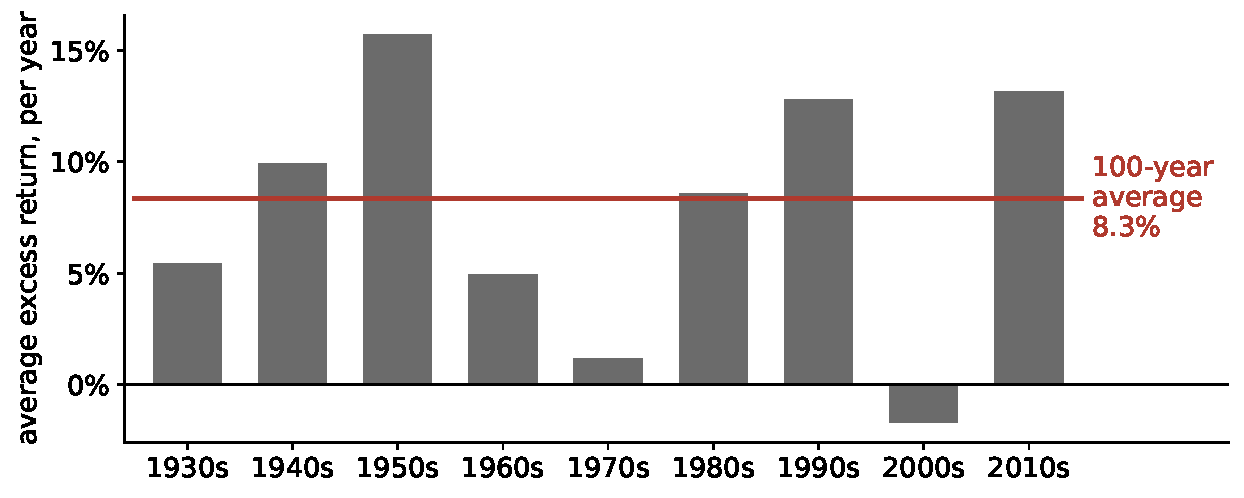
\includegraphics{figures/market_decades.pdf}}
\end{center}
\vskip 2pt
\begin{itemize}
\item 100 years: mean 8.3\%, volatility 18.4\%, Sharpe ratio 0.45
\vskip 6pt
\item After \emph{ten} years, the standard error of the mean is still \textcolor{red}{5.8\%}
\end{itemize}
\end{frame}

%------------------------------------------------------------------ 8
\begin{frame}{The arithmetic}
Each year's return has variance $\sigma^2$, and years are independent. The mean over $T$ years:
\[ \text{Var}\Big(\frac{1}{T}\sum_{t=1}^{T} r_t\Big) \;=\; \frac{1}{T^2} \times T\,\sigma^2 \;=\; \frac{\sigma^2}{T}
   \qquad\Longrightarrow\qquad \text{standard error} \;=\; \frac{\sigma}{\sqrt{T}} \]
\vskip 2pt
\[ t \;=\; \frac{\text{mean}}{\sigma/\sqrt{T}} \;=\; \text{ratio} \times \sqrt{T}
   \qquad\Longrightarrow\qquad T \;=\; \left(\frac{z}{\text{ratio}}\right)^{2} \]
\vskip 2pt
\begin{itemize}
\item \textbf{ratio}: the Sharpe ratio for a mean, the appraisal ratio for an alpha (annual)
\vskip 4pt
\item $z$: the $t$-statistic you require; $T$: years of data
\end{itemize}
\vskip 8pt
\begin{beamercolorbox}[rounded=true,sep=8pt,center]{box1}
The market: $(1.64 / 0.45)^2 = $ \textbf{13 years} to be 95\% sure its premium is above zero
\end{beamercolorbox}
\end{frame}

%------------------------------------------------------------------ 9
\begin{frame}{Years of data to reject zero}
\begin{center}
\renewcommand{\arraystretch}{1.25}
\begin{tabular}{lcccc}
\toprule
 & \multicolumn{4}{c}{$t$-statistic required} \\
\cmidrule(lr){2-5}
Sharpe or appraisal ratio & 1.64 & 1.96 & 2.58 & 3.00 \\
\midrule
0.30 & 30 & 43 & 74 & 100 \\
0.45 \;(the market) & \textcolor{red}{13} & 19 & 33 & 44 \\
0.50 & 11 & 15 & 27 & 36 \\
0.75 & 4.8 & 6.8 & 12 & 16 \\
1.00 & \textcolor{red}{2.7} & 3.8 & 6.7 & 9.0 \\
1.50 & 1.2 & 1.7 & 3.0 & 4.0 \\
2.00 & 0.7 & 1.0 & 1.7 & 2.3 \\
3.00 & 0.3 & 0.4 & 0.7 & 1.0 \\
\bottomrule
\end{tabular}
\end{center}
\vskip 4pt
\begin{itemize}
\item Halve the ratio and you need four times the data
\end{itemize}
\end{frame}

%------------------------------------------------------------------ 10
\begin{frame}{The same arithmetic, with a hurdle}
Divide by $\sigma$: the ratio itself has standard error $1/\sqrt{T}$. To show it is above a hurdle, not just above zero:
\vskip 6pt
\[ t \;=\; \frac{\text{ratio} - \text{hurdle}}{1/\sqrt{T}} \;=\; (\text{ratio} - \text{hurdle}) \times \sqrt{T}
   \qquad\Longrightarrow\qquad T \;=\; \left(\frac{z}{\text{ratio} - \text{hurdle}}\right)^{2} \]
\vskip 6pt
\begin{itemize}
\item Only the gap between the ratio and the hurdle counts
\vskip 6pt
\item A hurdle of zero gives back the formula you just used
\vskip 6pt
\item A ratio of 1 against a hurdle of 0.5: $(1.64 / 0.5)^2 = $ \textcolor{red}{11 years}
\end{itemize}
\end{frame}

%------------------------------------------------------------------ 11
\begin{frame}{Years to clear a hurdle}
\begin{center}
\renewcommand{\arraystretch}{1.25}
\begin{tabular}{lcccc}
\toprule
 & \multicolumn{4}{c}{to be 95\% sure the ratio is above} \\
\cmidrule(lr){2-5}
True ratio & 0 & 0.25 & 0.50 & 1.00 \\
\midrule
0.30 & 30 & 1,076 & --- & --- \\
0.50 & 11 & 43 & --- & --- \\
0.75 & 4.8 & 11 & 43 & --- \\
1.00 & 2.7 & 4.8 & \textcolor{red}{11} & --- \\
1.50 & 1.2 & 1.7 & 2.7 & 11 \\
2.00 & 0.7 & 0.9 & 1.2 & 2.7 \\
3.00 & 0.3 & 0.4 & 0.4 & 0.7 \\
\bottomrule
\end{tabular}
\end{center}
\vskip 4pt
\begin{itemize}
\item The closer the truth is to the bar, the longer it takes
\end{itemize}
\end{frame}

%------------------------------------------------------------------ 12
\begin{frame}{Beta and volatility are learned fast}
\begin{columns}[c]
\begin{column}{0.46\textwidth}
\adjustbox{max width=\textwidth, max height=0.74\textheight}{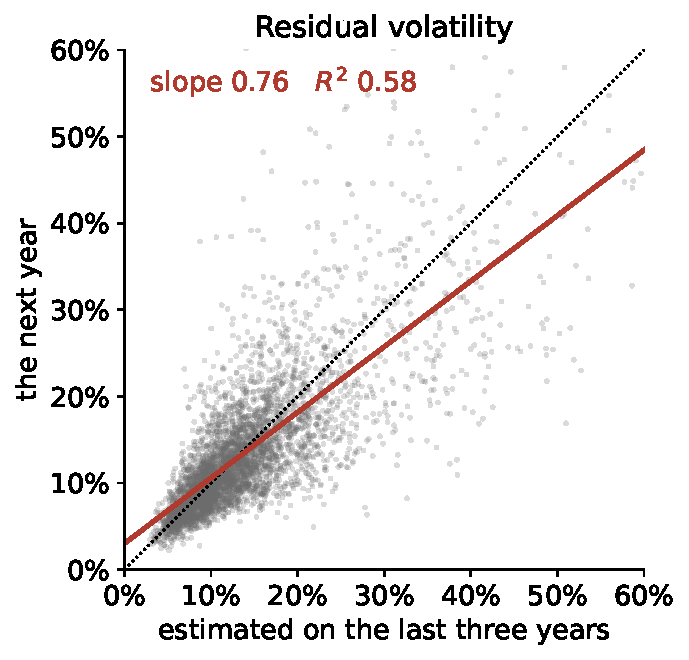
\includegraphics{figures/vol_persistence.pdf}}
\end{column}
\begin{column}{0.50\textwidth}
\begin{itemize}
\item Betas and volatilities are about how returns \emph{move}, not where they end up
\vskip 12pt
\item Their precision grows with the \textcolor{red}{number of observations}: sample daily, and months are enough
\vskip 12pt
\item A mean only gets sharper with calendar time
\end{itemize}
\end{column}
\end{columns}
\end{frame}

%------------------------------------------------------------------ 13
\begin{frame}{Frequency helps beta and volatility. The mean needs time.}
$T$ years of data, cut into $N$ observations. Daily instead of monthly: same $T$, 21 times the $N$.
\vskip 2pt
\begin{center}
\renewcommand{\arraystretch}{1.75}
\begin{tabular}{lll}
\toprule
 & standard error & shrinks with \\
\midrule
mean & $\sigma \,\big/ \sqrt{T}$ & \textcolor{red}{years} \\
alpha & $\sigma_\varepsilon \,\big/ \sqrt{T}$ & \textcolor{red}{years} \\
beta & $(\sigma_\varepsilon / \sigma_f) \,\big/ \sqrt{N}$ & observations \\
volatility & $\approx\; \sigma \,\big/ \sqrt{2N}$ & observations \\
\bottomrule
\end{tabular}
\end{center}
\vskip 2pt
\begin{itemize}
\item Three years of industry returns, monthly to daily: beta's standard error falls from \mbox{\textcolor{red}{0.14 to 0.03}}. Alpha's barely moves: 7.3\% to 6.9\%.
\vskip 5pt
\item The average return uses only the first price and the last. Looking in between adds nothing.
\end{itemize}
\end{frame}

%------------------------------------------------------------------ 14
\begin{frame}{Back to the factor model}
\[ r_t \;=\; \alpha \;+\; \beta\, f_t \;+\; \varepsilon_t \]
\vskip 6pt
\begin{center}
\renewcommand{\arraystretch}{1.5}
\begin{tabular}{llll}
\toprule
 & what it is & learned in & do recent past predicts future?\\
\midrule
$\beta$ & exposure to the factor & months & yes\\
$\sigma_\varepsilon$ & risk of its own & months & yes\\
$E[f]$ & factor  premium &decades  & no\\
$\sigma[f]$ & factor  vol &months  & yes\\
$\alpha$ & the edge & \textcolor{red}{decades?} & no \\
\bottomrule
\end{tabular}
\end{center}
\vskip 10pt
\begin{itemize}
\item The risk side of the model is knowable. The return side is the hard part.
\end{itemize}
\end{frame}

%------------------------------------------------------------------ 15
\begin{frame}[label=fleeting]{And alpha is fleeting}
\begin{itemize}
\item An edge that other people can see gets traded away
\vskip 14pt
\item So an alpha is a moving target: by the time the sample is long enough to measure it, it may be gone
\vskip 14pt
\item One more experiment
\end{itemize}
\end{frame}

%------------------------------------------------------------------ 16
\begin{frame}{Ideas cannot come from the data alone}
\begin{beamercolorbox}[rounded=true,sep=10pt,center]{box1}
You need \textbf{decades} of data to measure an alpha that may last only \textbf{years}.
\end{beamercolorbox}
\vskip 18pt
\begin{itemize}
\item So the data cannot be where the idea comes from
\vskip 12pt
\item The reason comes first: who is on the other side, and why are they paying you?
\vskip 12pt
\item Then the data tests it
\end{itemize}
\end{frame}

%------------------------------------------------------------------ 17
\begin{frame}{Estimate, tune, test}
\begin{center}
\renewcommand{\arraystretch}{1.6}
\begin{tabular}{lll}
\toprule
sample & what you do with it & may you look? \\
\midrule
\textbf{Estimate} & fit: the alphas, the betas, the ranking & yes \\
\textbf{Tune} & choose among your rules & yes \\
\textbf{Test} & report & \textcolor{red}{once, at the end} \\
\bottomrule
\end{tabular}
\end{center}
\vskip 12pt
\begin{beamercolorbox}[rounded=true,sep=8pt,center]{box1}
One question: are my estimates stable enough to trade on data they have not seen?
\end{beamercolorbox}
\vskip 8pt
\begin{itemize}
\item The experiment was exactly this: estimate on three years, test on the next
\end{itemize}
\end{frame}

%------------------------------------------------------------------ 18
\begin{frame}{How long should each window be?}
\begin{center}
\renewcommand{\arraystretch}{1.6}
\begin{tabular}{lll}
\toprule
window & long enough that & so check \\
\midrule
\textbf{Estimate} & the parameters are measured well & their standard errors \\
\textbf{Tune} & the metric you choose on is measured well & or you are choosing on noise \\
\textbf{Test} & the verdict is not noise & the standard error of the result \\
\bottomrule
\end{tabular}
\end{center}
\vskip 14pt
\begin{itemize}
\item In every window, a ratio measured over $T$ years has a standard error of about \textcolor{red}{$1/\sqrt{T}$}
\end{itemize}
\end{frame}

%------------------------------------------------------------------ 19
\begin{frame}{An example: looking for an appraisal ratio of 1}
You want to be 95\% sure the appraisal ratio is above zero.
\vskip 8pt
\[ T \;=\; \left(\frac{1.64}{\text{ratio} - \text{hurdle}}\right)^{2} \;=\; \left(\frac{1.64}{1 - 0}\right)^{2} \;=\; 2.7 \text{ years} \]
\vskip 8pt
\begin{beamercolorbox}[rounded=true,sep=8pt,center]{box1}
2.7 years in \emph{each} window: about \textbf{8 years} of data in all
\end{beamercolorbox}
\vskip 12pt

\end{frame}

%------------------------------------------------------------------ 20
\begin{frame}{Years of data you need, all three windows}
\begin{center}
\renewcommand{\arraystretch}{1.25}
\begin{tabular}{lcccc}
\toprule
 & \multicolumn{4}{c}{to be 95\% sure the ratio is above} \\
\cmidrule(lr){2-5}
True appraisal ratio & 0 & 0.25 & 0.50 & 1.00 \\
\midrule
0.50 & 32 & 129 & --- & --- \\
0.75 & 14 & 32 & 129 & --- \\
1.00 & \textcolor{red}{8.1} & 14 & 32 & --- \\
1.50 & 3.6 & 5.2 & 8.1 & 32 \\
2.00 & 2.0 & 2.6 & 3.6 & 8.1 \\
3.00 & 0.9 & 1.1 & 1.3 & 2.0 \\
\bottomrule
\end{tabular}
\end{center}
\vskip 4pt
\begin{itemize}
\item The notebook has 21 years, split 10 / 5 / 6: standard errors of 0.32, 0.45 and 0.41
\end{itemize}
\end{frame}

\begin{frame}[label=think]
	\begin{center}
		{\Large Something to think about}
	\end{center}
\end{frame}

\begin{frame}{The same experiment, with one year of data}
	Sorted into thirds here: buy the third with the highest $\alpha$, short the third with the lowest.
	\vskip 2pt
	\begin{center}
		\renewcommand{\arraystretch}{1.5}
		\begin{tabular}{lcccc}
			\toprule
			estimated on & alpha's standard error & promised & delivered next year & $t$ \\
			\midrule
			the last three years & 6.9\% & 20\% & 1.7\% & 1.6 \\
			the last year only & 11.6\% & 33\% & \textcolor{red}{4.4\%} & \textcolor{red}{4.2} \\
			\bottomrule
		\end{tabular}
	\end{center}
	\vskip 14pt
	\begin{itemize}
		\item A third of the data, and a noisier alpha
		\vskip 10pt
		\item Yet the trade earns more than twice as much
	\end{itemize}
	\vskip 6pt
	\hfill \hyperlink{fleeting}{\beamerreturnbutton{Back}}
\end{frame}

\begin{frame}{Rank on one year, then wait}
	\begin{center}
		\adjustbox{max width=0.92\textwidth, max height=0.60\textheight}{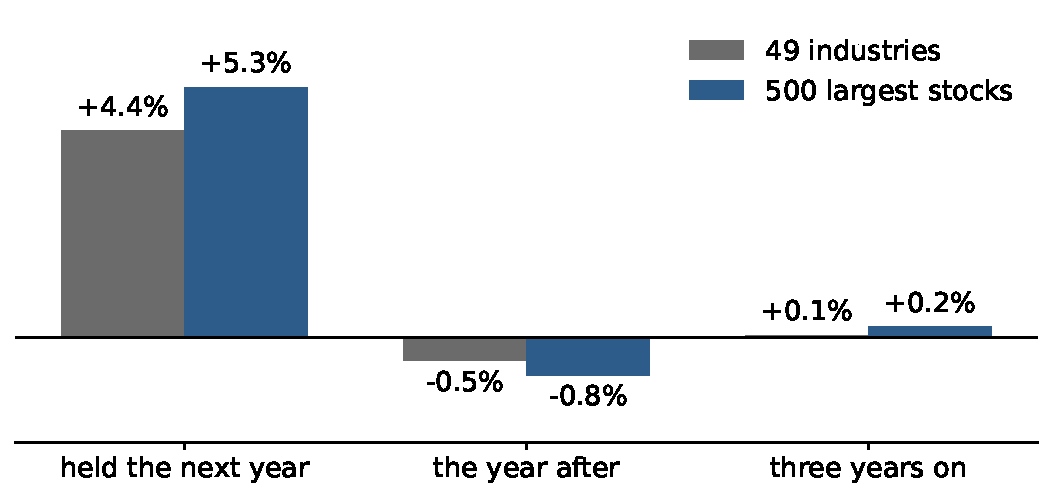
\includegraphics{figures/alpha_by_holding_year.pdf}}
	\end{center}
	\vskip 2pt
	\begin{itemize}
		\item Ranked on a single year: 4--5\% the next year, and nothing after that
	\end{itemize}
\end{frame}

\begin{frame}[label=think_stocks]{The same on the 500 largest stocks}
	\begin{center}
		\adjustbox{max width=\textwidth, max height=0.66\textheight}{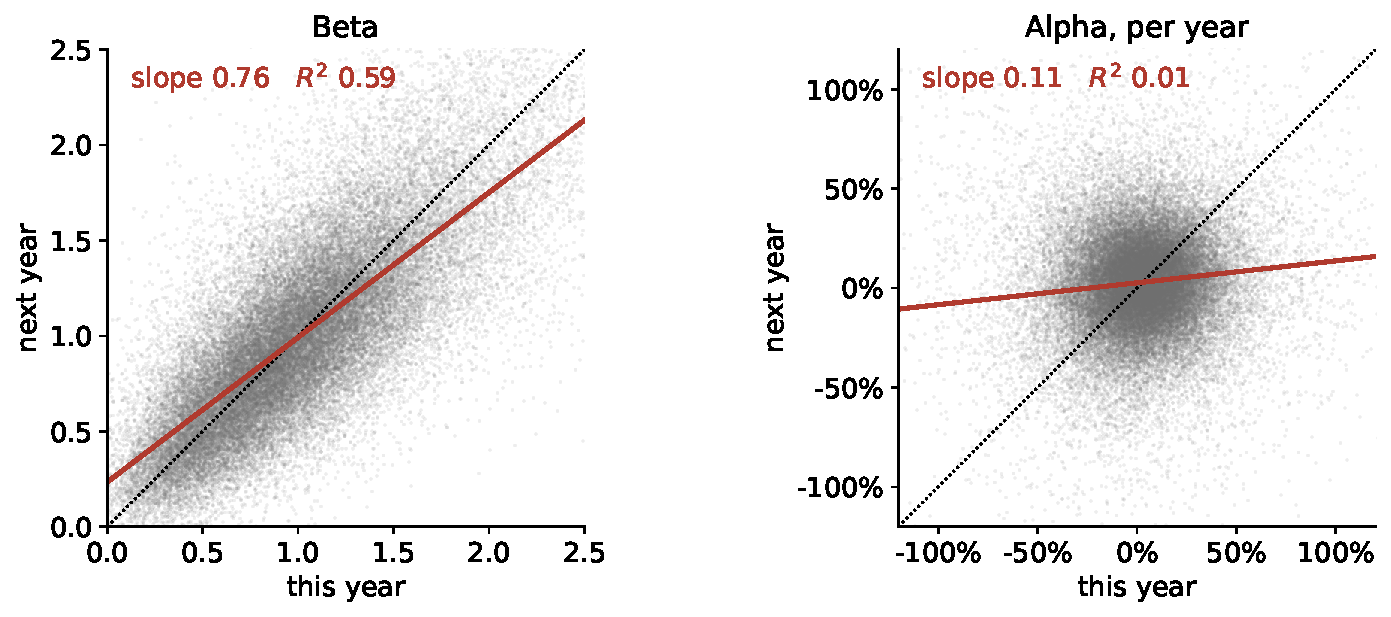
\includegraphics{figures/stock_beta_alpha_persistence.pdf}}
	\end{center}
	\vskip 2pt
	\begin{itemize}
		\item One year of data per stock: promised 53\%, delivered 5\% the next year
		\hfill \hyperlink{appendix_a2}{\beamerbutton{Details}}
	\end{itemize}
\end{frame}

\begin{frame}{What is going on?}
	\begin{beamercolorbox}[rounded=true,sep=10pt,center]{box1}
		How can a \textbf{smaller} sample lead to a \textbf{better} result?
	\end{beamercolorbox}
	\vskip 20pt
	\begin{itemize}
		\item Is alpha better measured with one year of data than with three?
		\vskip 14pt
		\item If not, what is going on?
	\end{itemize}
\end{frame}
%------------------------------------------------------------------ 21
\begin{frame}{Where this lives in the notebook}
\begin{center}
\renewcommand{\arraystretch}{1.6}
\begin{tabular}{ll}
\toprule
the idea & section of \emph{Backtesting: Estimate, Tune, Test} \\
\midrule
In-sample winners disappoint & Live demo: estimate $\rightarrow$ tune $\rightarrow$ test \\
A track record you could have lived through & 2. Walk-forward \\
How precisely a Sharpe ratio is measured & 3. What you report at the end \\
More attempts, higher bar & 5. You tried more than one \\
How long before you act & 7. When to start, and when to stop \\
\bottomrule
\end{tabular}
\end{center}
\vskip 10pt
\begin{itemize}
\item The code in each section computes one of these. Know which before you read it.
\end{itemize}
\end{frame}

%================================================================== appendix
\appendix
\begin{frame}
\begin{center}
{\Large Appendix}
\end{center}
\end{frame}

\begin{frame}[label=appendix_a1]{A1: How the experiment is built}
\begin{itemize}
\item \textbf{Data}: Ken French's 49 industry portfolios, daily returns, 1927--2025
\vskip 10pt
\item \textbf{Each December}: one regression per industry on the market, over the last three calendar years
\vskip 10pt
\item \textbf{The trade}: top fifth by estimated $\alpha$ minus bottom fifth, equal-weighted, held for the next year
\vskip 10pt
\item \textbf{The hedge}: each industry minus its estimated $\beta$ times the market
\vskip 10pt
\item No trading costs
\end{itemize}
\vskip 8pt
\hfill \hyperlink{experiment}{\beamerreturnbutton{Back}}
\end{frame}

\begin{frame}[label=appendix_a2]{A2: How the stock version is built}
\begin{itemize}
\item \textbf{Universe}: each year, the 500 largest US common stocks by market value at the end of the previous year (CRSP)
\vskip 10pt
\item \textbf{Regression}: daily returns within one calendar year, 1927--2025, delisting returns included
\vskip 10pt
\item \textbf{Same trade}: top third by $\alpha$ minus bottom third, hedged with the ranking year's $\beta$
\vskip 10pt
\item Each year's picks are followed for three more years, whether or not they stay in the top 500
\end{itemize}
\vskip 8pt
\hfill \hyperlink{think_stocks}{\beamerreturnbutton{Back}}
\end{frame}

%------------------------------------------------------------------ something to think about


\end{document}
